\chapter{परमाणु और अणु}\label{ch:g7:atoms-and-molecules}

पानी की एक बूँद लो और उसे दो हिस्सों में काटो। हर आधा हिस्सा अब भी पानी है।
आधे हिस्से को फिर दो में काटो, और फिर, और फिर। क्या तुम ऐसा हमेशा करते जा
सकते हो, या कभी ऐसा टुकड़ा मिलेगा जो इतना छोटा हो कि उसे एक बार और काटने पर
जो मिले वह पानी ही न रहे? ईसा पूर्व 400 के आसपास यूनानी
विचारक डेमोक्रिटस ने इसका उत्तर अनुमान से बताया: द्रव्य ऐसे नन्हे टुकड़ों से
बना है जिन्हें काटा नहीं जा सकता; उन्होंने उन्हें \emph{एटम} कहा, यूनानी में
``अविभाज्य''। उस अनुमान को विज्ञान बनने में दो हज़ार से ज़्यादा साल लगे, और
उन्नीसवीं सदी के रसायनज्ञों का काम भी। यह अध्याय इन टुकड़ों ---
\omterm{def:g7:atoms-and-molecules:atom}{परमाणुओं} --- का वर्णन करता है, और बताता है कि वे मिलकर
\omterm{def:g7:atoms-and-molecules:molecule}{अणु} कैसे बनाते हैं।

\begin{recall}
पानी या ऑक्सीजन जैसा \omterm{def:g6:pure-substances-and-mixtures:pure-substance}{शुद्ध पदार्थ} केवल एक ही \omterm{def:g6:pure-substances-and-mixtures:species}{रासायनिक स्पीशीज़} से बना होता
है; \omterm{def:g4:air-a-mixture-of-gases:air}{वायु} जैसे \omterm{def:g6:pure-substances-and-mixtures:mixture}{मिश्रण} में कई होती हैं
(\cref{ch:g6:pure-substances-and-mixtures})। \omterm{def:g4:air-a-mixture-of-gases:air}{वायु} लगभग चार-पाँचवाँ भाग
नाइट्रोजन और पाँचवाँ भाग ऑक्सीजन है (\cref{ch:g4:air-a-mixture-of-gases})।
\end{recall}

\section{परमाणु}

\begin{definition}[परमाणु]\label{def:g7:atoms-and-molecules:atom}
सारा द्रव्य बहुत ही छोटे कणों से बना है, जिन्हें
\emph{परमाणु}\index{परमाणु} कहते हैं। प्रकृति में परमाणुओं के केवल लगभग सौ
अलग-अलग प्रकार हैं, और हर पदार्थ --- पानी, \omterm{def:g4:air-a-mixture-of-gases:air}{वायु}, लोहा,
चीनी, हमारा अपना शरीर --- इनमें से कुछ प्रकारों के परमाणुओं से बना है।
\end{definition}

\begin{proposition}[परमाणु बहुत छोटे होते हैं]\label{prop:g7:atoms-and-molecules:tiny}
% ledger: const:a0, earth:diameter (8 cm apple: 12756 km / 8 cm = 1.6 x 10^8;
% 0.1-0.15 nm x 1.6 x 10^8 = 1.7-2.4 cm, a small cherry)
सबसे छोटा \omterm{def:g7:atoms-and-molecules:atom}{परमाणु}, हाइड्रोजन \omterm{def:g7:atoms-and-molecules:atom}{परमाणु}, आर-पार लगभग एक मिलीमीटर के करोड़वें भाग
जितना होता है; बाकी अधिक से अधिक कुछ गुना बड़े होते हैं। एक करोड़
हाइड्रोजन \omterm{def:g7:atoms-and-molecules:atom}{परमाणु} एक पंक्ति में रखें, तो एक मिलीमीटर लंबी रेखा बनेगी।
इसकी कल्पना ऐसे करो: अगर एक सेब को फुलाकर पृथ्वी जितना बड़ा कर दिया जाए, तो
उसका हर \omterm{def:g7:atoms-and-molecules:atom}{परमाणु} लगभग एक छोटी चेरी जितना होगा।
\end{proposition}

\begin{remark}[बिना दिखे देखा गया]\label{rem:g7:atoms-and-molecules:seen}
प्रकाश से काम करने वाला कोई भी सूक्ष्मदर्शी \omterm{def:g7:atoms-and-molecules:atom}{परमाणु} को नहीं दिखा सकता: \omterm{def:g7:atoms-and-molecules:atom}{परमाणु}
प्रकाश की तरंगों से बहुत छोटे होते हैं। 1980 के दशक से ऐसे विशेष सूक्ष्मदर्शी
बने हैं जो एक बेहद बारीक नोक से किसी सतह को टटोलते हैं; उनसे बने चित्रों में
अकेले \omterm{def:g7:atoms-and-molecules:atom}{परमाणु} उभारों की तरह दिखते हैं।
\end{remark}

\begin{definition}[परमाणु का प्रतीक]\label{def:g7:atoms-and-molecules:symbol}
हर प्रकार के \omterm{def:g7:atoms-and-molecules:atom}{परमाणु} का एक नाम और एक \emph{प्रतीक}\index{परमाणु का प्रतीक} होता है:
एक बड़ा (कैपिटल) अक्षर, जिसके बाद कभी-कभी एक छोटा अक्षर आता है।
प्रतीक हर भाषा में एक ही होता है।
\end{definition}

\begin{center}
\small
\begin{tabular}{llll|llll}
\hline
\omterm{def:g7:atoms-and-molecules:atom}{परमाणु} & \omterm{def:g7:atoms-and-molecules:symbol}{प्रतीक} & & मॉडल का रंग & \omterm{def:g7:atoms-and-molecules:atom}{परमाणु} & \omterm{def:g7:atoms-and-molecules:symbol}{प्रतीक} & & मॉडल का रंग \\
\hline
हाइड्रोजन & \ce{H} & \tikz\node[aH]{}; & सफ़ेद & सोडियम & \ce{Na} & \tikz\node[aNa]{}; & बैंगनी \\
कार्बन & \ce{C} & \tikz\node[aC]{}; & काला & सल्फ़र & \ce{S} & \tikz\node[aS]{}; & पीला \\
नाइट्रोजन & \ce{N} & \tikz\node[aN]{}; & नीला & क्लोरीन & \ce{Cl} & \tikz\node[aCl]{}; & हरा \\
ऑक्सीजन & \ce{O} & \tikz\node[aO]{}; & लाल & लोहा, ताँबा & \ce{Fe}, \ce{Cu} & & --- \\
\hline
\end{tabular}
\end{center}

\begin{remark}[प्रतीक कहाँ से आते हैं]\label{rem:g7:atoms-and-molecules:latin}
ज़्यादातर \omterm{def:g7:atoms-and-molecules:symbol}{प्रतीक} अंग्रेज़ी नाम के पहले अक्षर हैं: हाइड्रोजन के लिए \ce{H},
कार्बन के लिए \ce{C}, ऑक्सीजन के लिए \ce{O}। कुछ एक पुराने, लैटिन
नाम से आते हैं: सोडियम के लिए \ce{Na} (\emph{नेट्रियम}), लोहे के लिए \ce{Fe}
(\emph{फ़ेरम}), ताँबे के लिए \ce{Cu} (\emph{क्यूप्रम})। दूसरा अक्षर
हमेशा छोटा होता है: \ce{Co} कोबाल्ट \omterm{def:g7:atoms-and-molecules:atom}{परमाणु} है, जबकि बड़े O वाला CO
बिल्कुल अलग चीज़ है।
\end{remark}

\begin{history}[डाल्टन के परमाणु, 1808]
1808 में रसायनज्ञ जॉन डाल्टन ने उस समय ज्ञात \omterm{def:g7:atoms-and-molecules:atom}{परमाणुओं} की एक सारणी प्रकाशित
की, जिसमें हर \omterm{def:g7:atoms-and-molecules:atom}{परमाणु} को अपने अलग चिह्न वाले एक छोटे वृत्त के रूप में बनाया
गया था। उन्होंने सबसे पहले कहा कि एक प्रकार के हर \omterm{def:g7:atoms-and-molecules:atom}{परमाणु} का भार एक ही होता है,
और रसायनज्ञ इन भारों की तुलना कर सकते हैं। पर उन्होंने यह भी अनुमान लगाया कि
पानी एक हाइड्रोजन \omterm{def:g7:atoms-and-molecules:atom}{परमाणु} और एक ऑक्सीजन \omterm{def:g7:atoms-and-molecules:atom}{परमाणु} के जुड़ने से बना है; रसायनज्ञों
को यह मानने में और पचास साल लगे कि पानी के \omterm{def:g7:atoms-and-molecules:molecule}{अणु} में \emph{दो}
हाइड्रोजन \omterm{def:g7:atoms-and-molecules:atom}{परमाणु} होते हैं।
\end{history}

\begin{omfigure}
\begin{minipage}[b]{0.3\linewidth}\centering
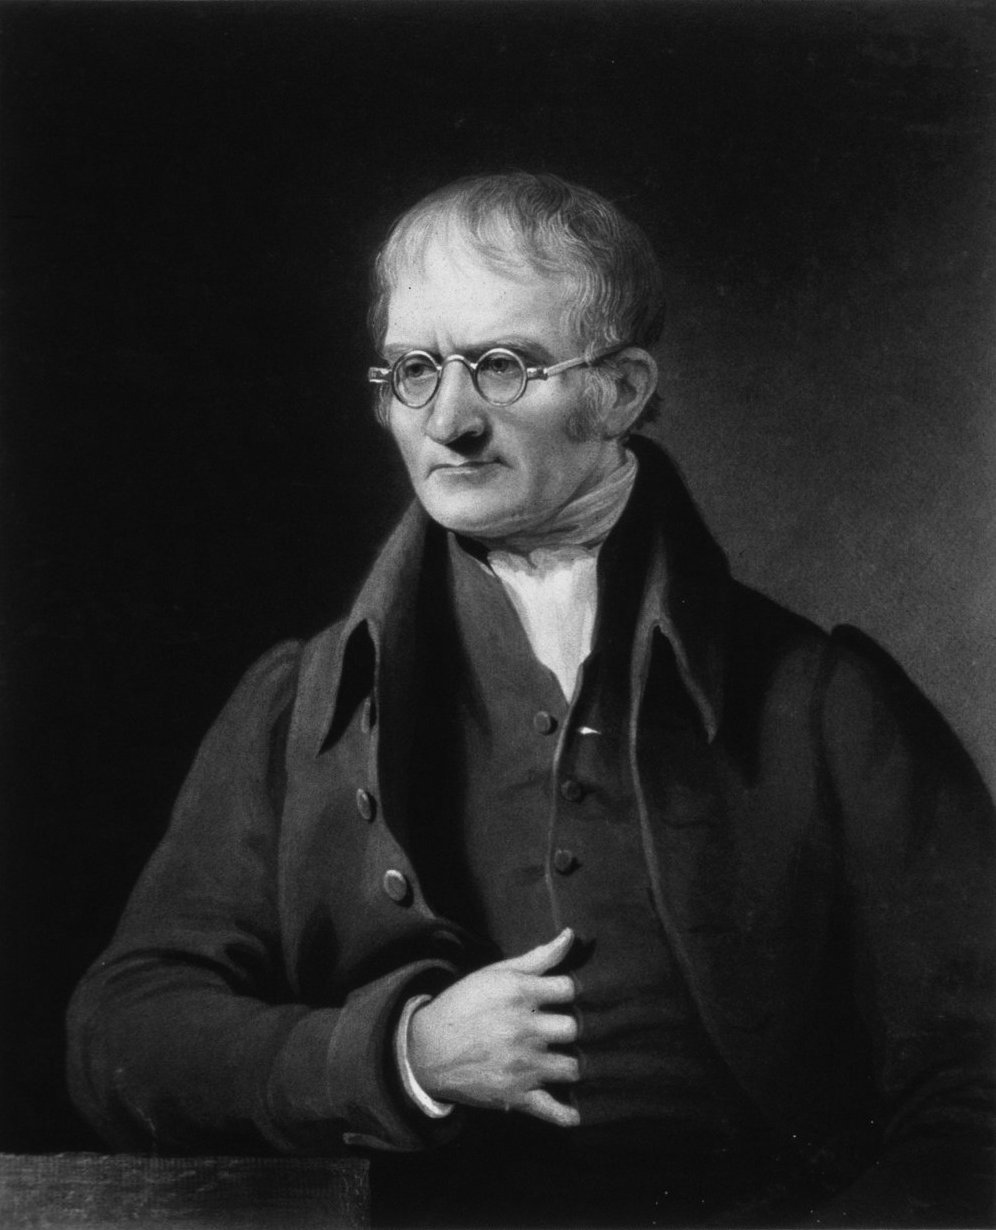
\includegraphics[width=\linewidth]{images/book1/dalton.jpg}

{\small जॉन डाल्टन (1766--1844)।}
\end{minipage}\hfill
\begin{minipage}[b]{0.66\linewidth}\centering
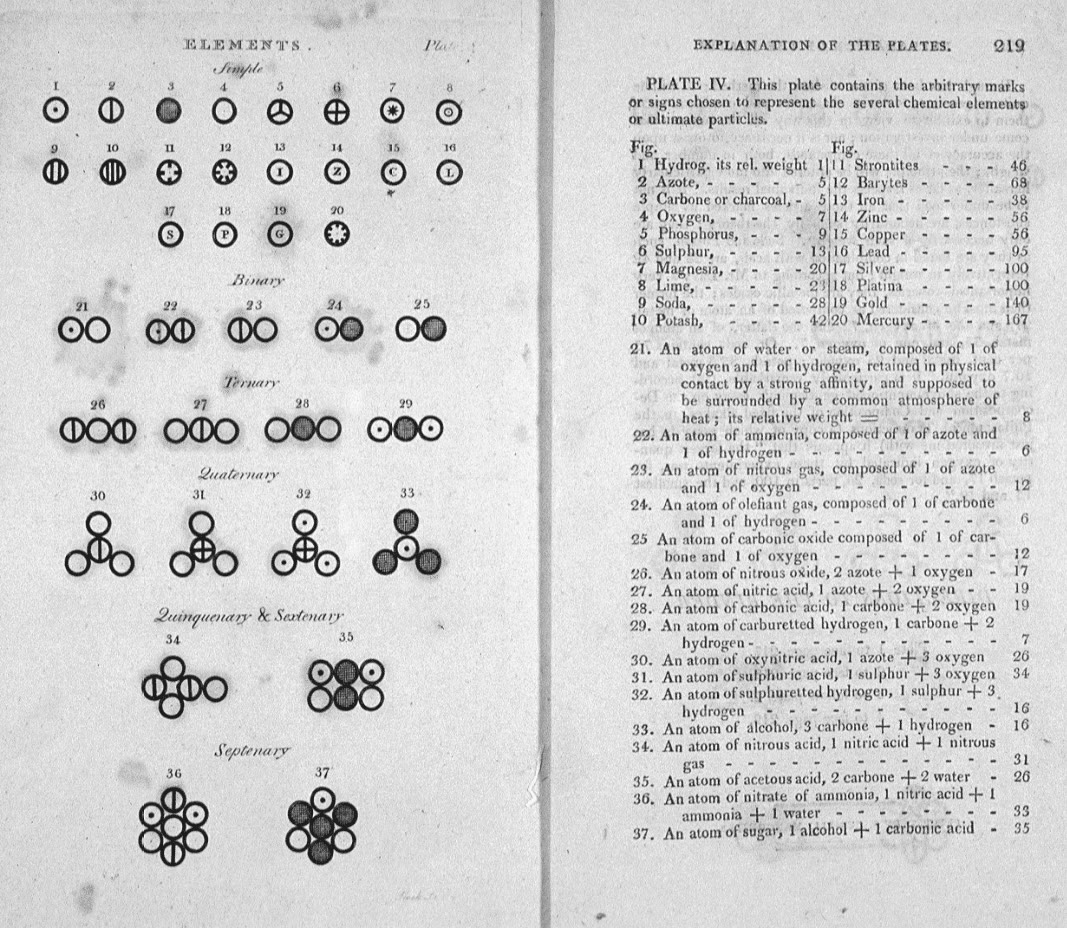
\includegraphics[width=\linewidth]{images/book1/dalton-symbols.jpg}

{\small डाल्टन की 1808 की सारणी: उनका पानी, चिह्न 21, हाइड्रोजन के एक वृत्त
के बगल में ऑक्सीजन का एक वृत्त है।}
\end{minipage}
\end{omfigure}

\section{अणु}

\begin{definition}[अणु]\label{def:g7:atoms-and-molecules:molecule}
\emph{अणु}\index{अणु} \omterm{def:g7:atoms-and-molecules:atom}{परमाणुओं} का एक समूह है जो आपस में मज़बूती से
जुड़ा रहता है। अणु किसी पदार्थ का वह सबसे छोटा टुकड़ा है जो अब भी वही
पदार्थ है: पानी का एक अणु पानी की सबसे छोटी संभव
मात्रा है।
\end{definition}

\begin{example}[सात अणु]\label{ex:g7:atoms-and-molecules:seven}
\begin{itemize}
  \item \emph{हाइड्रोजन} का \omterm{def:g7:atoms-and-molecules:molecule}{अणु}: दो हाइड्रोजन \omterm{def:g7:atoms-and-molecules:atom}{परमाणु};
  \item \emph{ऑक्सीजन} का \omterm{def:g7:atoms-and-molecules:molecule}{अणु}, जिसे हम साँस में लेते हैं: दो ऑक्सीजन \omterm{def:g7:atoms-and-molecules:atom}{परमाणु};
  \item \emph{नाइट्रोजन} का \omterm{def:g7:atoms-and-molecules:molecule}{अणु}, \omterm{def:g4:air-a-mixture-of-gases:air}{वायु} का चार-पाँचवाँ भाग: दो
        नाइट्रोजन \omterm{def:g7:atoms-and-molecules:atom}{परमाणु};
  \item \emph{पानी} का \omterm{def:g7:atoms-and-molecules:molecule}{अणु}: दो हाइड्रोजन \omterm{def:g7:atoms-and-molecules:atom}{परमाणु} और एक ऑक्सीजन
        \omterm{def:g7:atoms-and-molecules:atom}{परमाणु};
  \item \emph{कार्बन डाइऑक्साइड} का \omterm{def:g7:atoms-and-molecules:molecule}{अणु}, जिसे हम बाहर छोड़ते हैं: एक
        कार्बन \omterm{def:g7:atoms-and-molecules:atom}{परमाणु} और दो ऑक्सीजन \omterm{def:g7:atoms-and-molecules:atom}{परमाणु};
  \item \emph{मेथेन} का \omterm{def:g7:atoms-and-molecules:molecule}{अणु}, गैस चूल्हों में \omterm{def:g4:what-a-fire-needs:burning}{जलने} वाली प्राकृतिक गैस का
        मुख्य भाग: एक कार्बन \omterm{def:g7:atoms-and-molecules:atom}{परमाणु} और चार हाइड्रोजन \omterm{def:g7:atoms-and-molecules:atom}{परमाणु};
  \item \emph{नाइट्रस ऑक्साइड} का \omterm{def:g7:atoms-and-molecules:molecule}{अणु}, एक निश्चेतक गैस: दो
        नाइट्रोजन \omterm{def:g7:atoms-and-molecules:atom}{परमाणु} और एक ऑक्सीजन \omterm{def:g7:atoms-and-molecules:atom}{परमाणु}।
\end{itemize}
\end{example}

\begin{omfigure}
\begin{tikzpicture}[font=\small]
  % hydrogen
  \begin{scope}[xshift=0cm]
    \node[aH] (a) at (-0.25,0) {}; \node[aH] (b) at (0.25,0) {};
    \begin{scope}[on background layer]\draw[bond] (a.center) -- (b.center);\end{scope}
    \node at (0,-1.05) {हाइड्रोजन};
  \end{scope}
  % oxygen
  \begin{scope}[xshift=2.6cm]
    \node[aO] (a) at (-0.33,0) {}; \node[aO] (b) at (0.33,0) {};
    \begin{scope}[on background layer]
      \draw[bond, line width=1.1pt] ([yshift=1.6pt]a.center) -- ([yshift=1.6pt]b.center);
      \draw[bond, line width=1.1pt] ([yshift=-1.6pt]a.center) -- ([yshift=-1.6pt]b.center);
    \end{scope}
    \node at (0,-1.05) {ऑक्सीजन};
  \end{scope}
  % nitrogen
  \begin{scope}[xshift=5.2cm]
    \node[aN] (a) at (-0.33,0) {}; \node[aN] (b) at (0.33,0) {};
    \begin{scope}[on background layer]
      \foreach \d in {-2.4,0,2.4}
        \draw[bond, line width=0.9pt] ([yshift=\d pt]a.center) -- ([yshift=\d pt]b.center);
    \end{scope}
    \node at (0,-1.05) {नाइट्रोजन};
  \end{scope}
  % water
  \begin{scope}[xshift=7.8cm, yshift=0.2cm]
    \node[aO] (o) at (0,0) {};
    \node[aH] (h1) at (-0.62,-0.48) {}; \node[aH] (h2) at (0.62,-0.48) {};
    \begin{scope}[on background layer]
      \draw[bond] (o.center) -- (h1.center); \draw[bond] (o.center) -- (h2.center);
    \end{scope}
    \node at (0,-1.25) {पानी};
  \end{scope}
  % carbon dioxide
  \begin{scope}[xshift=0.9cm, yshift=-2.7cm]
    \node[aO] (a) at (-0.85,0) {}; \node[aC] (c) at (0,0) {}; \node[aO] (b) at (0.85,0) {};
    \begin{scope}[on background layer]
      \foreach \d in {-1.6,1.6} {
        \draw[bond, line width=1.1pt] ([yshift=\d pt]a.center) -- ([yshift=\d pt]c.center);
        \draw[bond, line width=1.1pt] ([yshift=\d pt]c.center) -- ([yshift=\d pt]b.center);}
    \end{scope}
    \node at (0,-1.05) {कार्बन डाइऑक्साइड};
  \end{scope}
  % methane
  \begin{scope}[xshift=4.4cm, yshift=-2.6cm]
    \node[aC] (c) at (0,0) {};
    \node[aH] (h1) at (0,0.78) {};
    \node[aH] (h2) at (-0.74,-0.3) {};
    \node[aH] (h3) at (0.74,-0.3) {};
    \begin{scope}[on background layer]
      \draw[bond] (c.center) -- (h1.center); \draw[bond] (c.center) -- (h2.center);
      \draw[bond] (c.center) -- (h3.center);
    \end{scope}
    \draw[bond] (c.center) -- (0.22,-0.52);
    \node[aH] at (0.24,-0.58) {};
    \node at (0,-1.15) {मेथेन};
  \end{scope}
  % nitrous oxide
  \begin{scope}[xshift=7.8cm, yshift=-2.7cm]
    \node[aN] (a) at (-0.8,0) {}; \node[aN] (b) at (0,0) {}; \node[aO] (c) at (0.8,0) {};
    \begin{scope}[on background layer]
      \foreach \d in {-1.6,1.6} {
        \draw[bond, line width=1.1pt] ([yshift=\d pt]a.center) -- ([yshift=\d pt]b.center);
        \draw[bond, line width=1.1pt] ([yshift=\d pt]b.center) -- ([yshift=\d pt]c.center);}
    \end{scope}
    \node at (0,-1.05) {नाइट्रस ऑक्साइड};
  \end{scope}
\end{tikzpicture}

{\small \cref{ex:g7:atoms-and-molecules:seven} के सात \omterm{def:g7:atoms-and-molecules:molecule}{अणुओं} के
गेंद-और-छड़ मॉडल। हर छड़ दो \omterm{def:g7:atoms-and-molecules:atom}{परमाणुओं} के बीच के एक आबंध को दिखाती है; कुछ
\omterm{def:g7:atoms-and-molecules:atom}{परमाणु} दो या तीन छड़ें क्यों साझा करते हैं, यह आगे के एक अध्याय में समझाया
गया है।}
\end{omfigure}

\begin{proposition}[शुद्ध पदार्थ और मिश्रण के अणु]\label{prop:g7:atoms-and-molecules:pure}
\omterm{def:g7:atoms-and-molecules:molecule}{अणुओं} से बने \omterm{def:g6:pure-substances-and-mixtures:pure-substance}{शुद्ध पदार्थ} में सभी \omterm{def:g7:atoms-and-molecules:molecule}{अणु} एक जैसे होते हैं:
शुद्ध पानी में केवल पानी के \omterm{def:g7:atoms-and-molecules:molecule}{अणु} होते हैं। \omterm{def:g6:pure-substances-and-mixtures:mixture}{मिश्रण} में कई प्रकार के \omterm{def:g7:atoms-and-molecules:molecule}{अणु} होते
हैं: \omterm{def:g4:air-a-mixture-of-gases:air}{वायु} ज़्यादातर नाइट्रोजन के \omterm{def:g7:atoms-and-molecules:molecule}{अणु} और ऑक्सीजन के \omterm{def:g7:atoms-and-molecules:molecule}{अणु} है, ऑक्सीजन के हर
एक \omterm{def:g7:atoms-and-molecules:molecule}{अणु} पर लगभग चार नाइट्रोजन के, साथ में कुछ आर्गन \omterm{def:g7:atoms-and-molecules:atom}{परमाणु} जो अकेले रहते
हैं, और कार्बन डाइऑक्साइड के बहुत कम \omterm{def:g7:atoms-and-molecules:molecule}{अणु}।
\end{proposition}

\begin{omfigure}
\begin{tikzpicture}[font=\small,
    sN/.style={aN, minimum size=3.0mm}, sO/.style={aO, minimum size=2.9mm},
    sH/.style={aH, minimum size=2.1mm}, sAr/.style={om atom, ball color=cyan!60, minimum size=3.4mm}]
  % air
  \draw[omGlass, line width=0.6pt] (0,0) rectangle (3.4,3.4);
  \foreach \x/\y/\r in {0.5/0.6/20, 1.6/0.4/-30, 2.8/0.7/75, 0.6/1.7/110,
                        2.0/1.5/10, 2.9/2.0/-60, 0.9/2.8/40, 2.1/2.9/-15}
    \node[sN] at ($(\x,\y)+(\r:0.12)$) {} node[sN] at ($(\x,\y)+(\r+180:0.12)$) {};
  \foreach \x/\y/\r in {1.3/1.1/60, 1.6/2.3/-40}
    \node[sO] at ($(\x,\y)+(\r:0.12)$) {} node[sO] at ($(\x,\y)+(\r+180:0.12)$) {};
  \node[sAr] at (2.9,3.0) {};
  \node[anchor=north] at (1.7,-0.1) {\textbf{वायु}: एक मिश्रण};
  % water
  \begin{scope}[xshift=5.2cm]
    \draw[omGlass, line width=0.6pt] (0,0) rectangle (3.4,3.4);
    \foreach \x in {0,1,2,3,4} \foreach \y in {0,1,2,3,4} {
      \pgfmathsetmacro{\ang}{mod(73*\x+41*\y,360)}
      \begin{scope}[shift={({0.36+0.67*\x},{0.4+0.66*\y})}, rotate=\ang]
        \node[sH] at (-0.16,-0.12) {}; \node[sH] at (0.16,-0.12) {};
        \node[sO] at (0,0) {};
      \end{scope}}
    \node[anchor=north] at (1.7,-0.1) {\textbf{पानी}: एक शुद्ध पदार्थ};
  \end{scope}
\end{tikzpicture}

{\small बहुत अधिक आवर्धन करके देखना। बाएँ: \omterm{def:g4:air-a-mixture-of-gases:air}{वायु} में नाइट्रोजन के \omterm{def:g7:atoms-and-molecules:molecule}{अणु} (नीले)
ऑक्सीजन के \omterm{def:g7:atoms-and-molecules:molecule}{अणुओं} (लाल) से कहीं ज़्यादा हैं, और एक आर्गन \omterm{def:g7:atoms-and-molecules:atom}{परमाणु} (हल्का
नीला) अकेला घूमता है; गैस के \omterm{def:g7:atoms-and-molecules:molecule}{अणु} एक-दूसरे से दूर होते हैं। दाएँ: द्रव पानी
में सभी \omterm{def:g7:atoms-and-molecules:molecule}{अणु} एक जैसे हैं और एक-दूसरे को छूते हैं।}
\end{omfigure}

\section{रासायनिक सूत्र}

\begin{definition}[रासायनिक सूत्र]\label{def:g7:atoms-and-molecules:formula}
किसी \omterm{def:g7:atoms-and-molecules:molecule}{अणु} का \emph{रासायनिक सूत्र}\index{रासायनिक सूत्र} उसके \omterm{def:g7:atoms-and-molecules:atom}{परमाणुओं} के
प्रतीकों की सूची है, जिसमें हर \omterm{def:g7:atoms-and-molecules:symbol}{प्रतीक} के बाद रेखा के नीचे लिखी एक छोटी संख्या
आती है --- यह \emph{पादांक}\index{पादांक} है --- जो बताती है कि \omterm{def:g7:atoms-and-molecules:molecule}{अणु} में उस
प्रकार के कितने \omterm{def:g7:atoms-and-molecules:atom}{परमाणु} हैं। पादांक 1 लिखा नहीं जाता।
\end{definition}

\begin{example}[सातों सूत्र]\label{ex:g7:atoms-and-molecules:formulas}
\cref{ex:g7:atoms-and-molecules:seven} के \omterm{def:g7:atoms-and-molecules:molecule}{अणुओं} के सूत्र
ये हैं:
\begin{center}
\begin{tabular}{lcl}
\hline
\omterm{def:g7:atoms-and-molecules:molecule}{अणु} & सूत्र & \omterm{def:g7:atoms-and-molecules:atom}{परमाणु} \\
\hline
हाइड्रोजन & \ce{H2} & 2 हाइड्रोजन \\
ऑक्सीजन & \ce{O2} & 2 ऑक्सीजन \\
नाइट्रोजन & \ce{N2} & 2 नाइट्रोजन \\
पानी & \ce{H2O} & 2 हाइड्रोजन, 1 ऑक्सीजन \\
कार्बन डाइऑक्साइड & \ce{CO2} & 1 कार्बन, 2 ऑक्सीजन \\
मेथेन & \ce{CH4} & 1 कार्बन, 4 हाइड्रोजन \\
नाइट्रस ऑक्साइड & \ce{N2O} & 2 नाइट्रोजन, 1 ऑक्सीजन \\
\hline
\end{tabular}
\end{center}
\end{example}

\begin{method}[सूत्र पढ़ना]\label{met:g7:atoms-and-molecules:read}
किसी \omterm{def:g7:atoms-and-molecules:molecule}{अणु} का सूत्र पढ़ने के लिए:
\begin{enumerate}
  \item उसे प्रतीकों में बाँटो: हर \omterm{def:g7:atoms-and-molecules:symbol}{प्रतीक} बड़े अक्षर से शुरू होता है;
  \item हर \omterm{def:g7:atoms-and-molecules:symbol}{प्रतीक} के बाद \omterm{def:g7:atoms-and-molecules:formula}{पादांक} पढ़ो (\omterm{def:g7:atoms-and-molecules:formula}{पादांक} न हो तो 1);
  \item \omterm{def:g7:atoms-and-molecules:atom}{परमाणुओं} की कुल संख्या पाने के लिए \omterm{def:g7:atoms-and-molecules:formula}{पादांकों} को जोड़ो।
\end{enumerate}
\ce{C2H6O} (एथेनॉल, पेयों में पाया जाने वाला ऐल्कोहॉल) के लिए: 2 कार्बन, 6 हाइड्रोजन,
1 ऑक्सीजन, कुल 9 \omterm{def:g7:atoms-and-molecules:atom}{परमाणु}।
\end{method}

\begin{remark}[आगे लिखी संख्या]\label{rem:g7:atoms-and-molecules:coefficient}
सूत्र के आगे लिखी संख्या \omterm{def:g7:atoms-and-molecules:molecule}{अणुओं} को गिनती है: \ce{3H2O} का अर्थ है
पानी के तीन \omterm{def:g7:atoms-and-molecules:molecule}{अणु}, जिनमें मिलाकर 6 हाइड्रोजन \omterm{def:g7:atoms-and-molecules:atom}{परमाणु} और 3 ऑक्सीजन
\omterm{def:g7:atoms-and-molecules:atom}{परमाणु} हैं। \ce{O2}, यानी दो ऑक्सीजन \omterm{def:g7:atoms-and-molecules:atom}{परमाणुओं} से बना एक \omterm{def:g7:atoms-and-molecules:molecule}{अणु}, को
\ce{2O} से न मिलाओ, जो दो ऑक्सीजन \omterm{def:g7:atoms-and-molecules:atom}{परमाणु} हैं जो जुड़े नहीं हैं।
\end{remark}

\begin{example}[रसोई में मेथेन]\label{ex:g7:atoms-and-molecules:methane}
गैस चूल्हे की प्राकृतिक गैस ज़्यादातर मेथेन, \ce{CH4}, है। उसका हर \omterm{def:g7:atoms-and-molecules:molecule}{अणु}
एक कार्बन \omterm{def:g7:atoms-and-molecules:atom}{परमाणु} है जिसके चारों ओर चार हाइड्रोजन \omterm{def:g7:atoms-and-molecules:atom}{परमाणु} हैं। यह गैस
अदृश्य और गंधहीन है: ``गैस'' की गंध एक ऐसे पदार्थ की है जो जान-बूझकर
मिलाया जाता है, ताकि रिसाव का पता चल जाए।
\end{example}

\begin{omfigure}
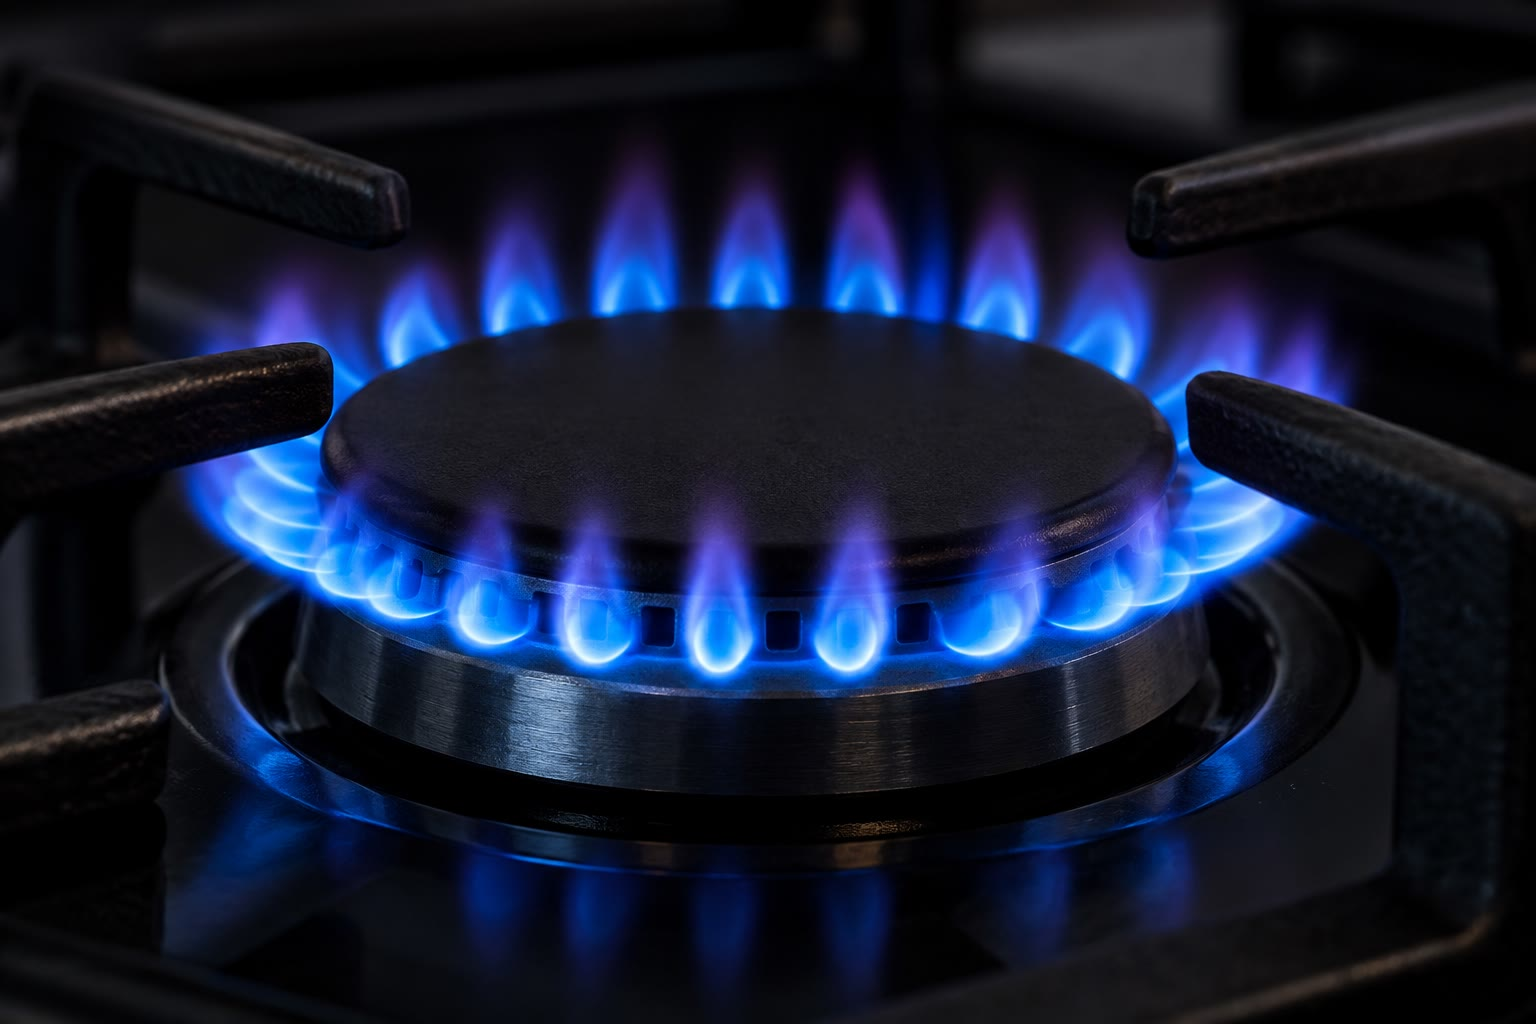
\includegraphics[width=0.5\linewidth]{images/book1/ai/g7-gas-flame.jpg}

{\small गैस चूल्हे की नीली लौ: प्राकृतिक गैस की मेथेन जल रही है।}
\end{omfigure}

\section{आण्विक मॉडल}

\begin{remark}[मॉडल, और उनके रंग]\label{rem:g7:atoms-and-molecules:models}
रसायनज्ञ \omterm{def:g7:atoms-and-molecules:atom}{परमाणुओं} के लिए गेंदों और उनके बीच के आबंधों के लिए छड़ों से
\emph{आण्विक मॉडल} बनाते हैं। ये रंग पूरी दुनिया में अपनाई गई एक
परिपाटी है --- कार्बन काला, हाइड्रोजन सफ़ेद, ऑक्सीजन लाल, नाइट्रोजन
नीला --- \omterm{def:g7:atoms-and-molecules:atom}{परमाणुओं} का असली रंग नहीं: एक अकेले \omterm{def:g7:atoms-and-molecules:atom}{परमाणु} का कोई रंग होता ही
नहीं। मॉडल \omterm{def:g7:atoms-and-molecules:molecule}{अणु} की आकृति भी दिखाता है, जो सूत्र नहीं दिखाता: पानी का \omterm{def:g7:atoms-and-molecules:molecule}{अणु}
मुड़ा हुआ है, कार्बन डाइऑक्साइड का \omterm{def:g7:atoms-and-molecules:molecule}{अणु}
सीधा।
\end{remark}

\begin{omfigure}
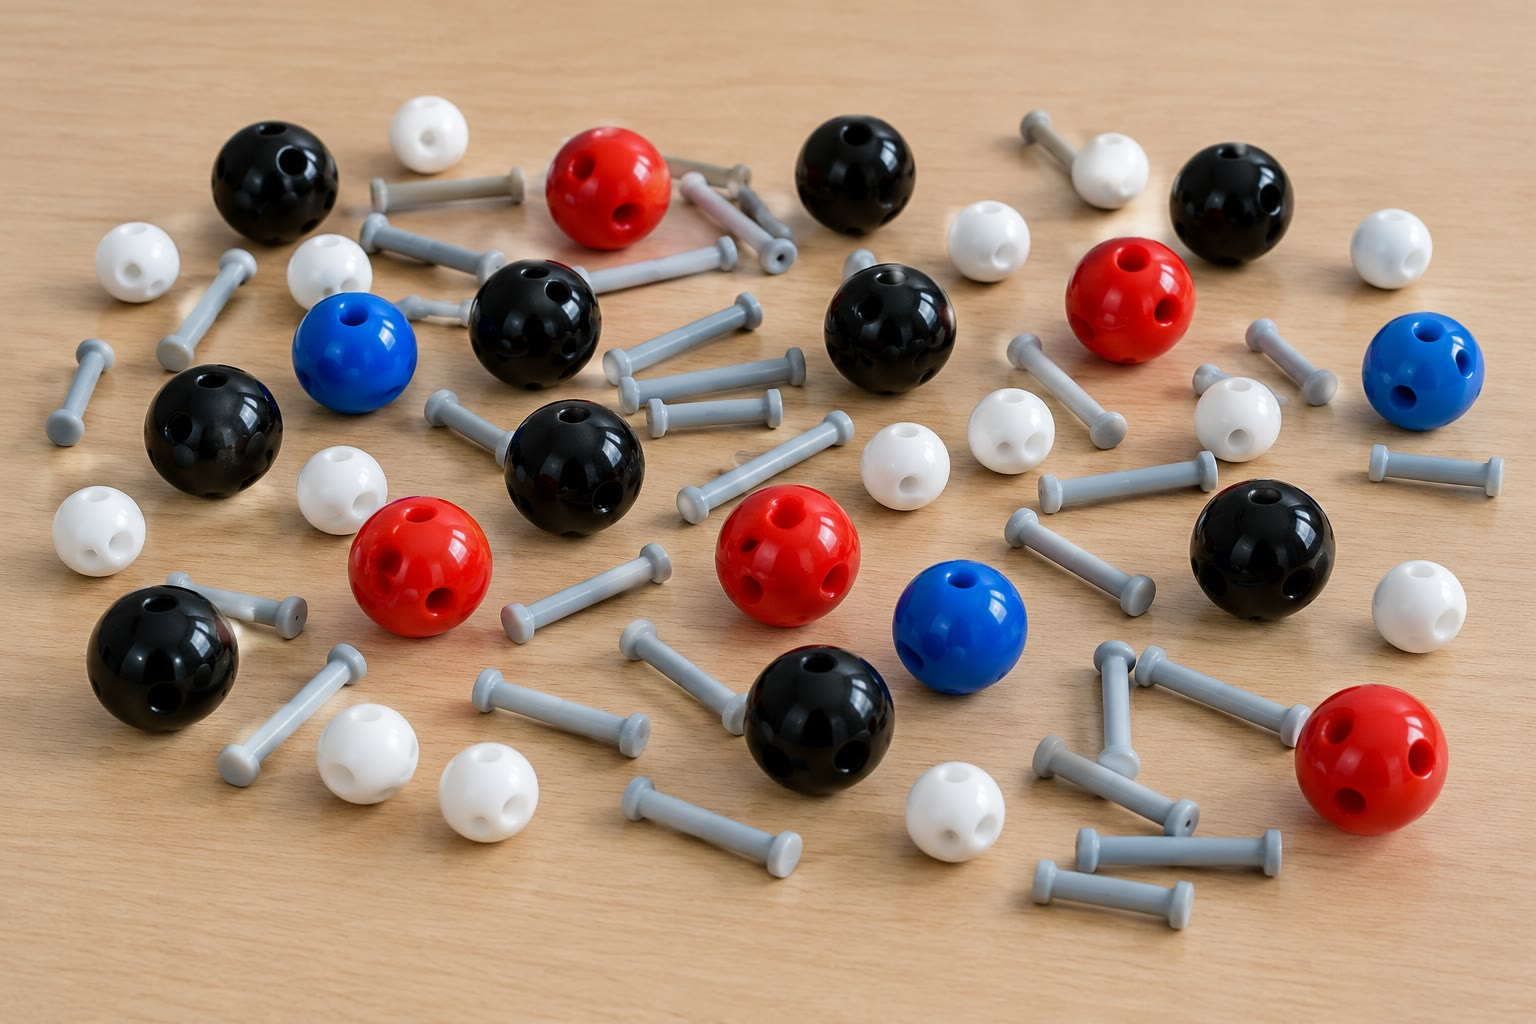
\includegraphics[width=0.5\linewidth]{images/book1/ai/g7-model-kit.jpg}

{\small आण्विक मॉडल किट: \omterm{def:g7:atoms-and-molecules:atom}{परमाणुओं} के लिए गेंदें, जिनमें आबंधों को दिखाने
वाली छड़ों के लिए छेद हैं।}
\end{omfigure}

\begin{method}[मॉडल से सूत्र तक]\label{met:g7:atoms-and-molecules:model}
किसी \omterm{def:g7:atoms-and-molecules:molecule}{अणु} का सूत्र उसके मॉडल से लिखने के लिए:
\begin{enumerate}
  \item रंगों से \omterm{def:g7:atoms-and-molecules:atom}{परमाणुओं} के नाम पहचानो;
  \item हर रंग की गेंदें गिनो;
  \item प्रतीकों को गिनती के \omterm{def:g7:atoms-and-molecules:formula}{पादांकों} के साथ लिखो: पहले कार्बन, फिर
        हाइड्रोजन, फिर बाकी \omterm{def:g7:atoms-and-molecules:atom}{परमाणु} अपने प्रतीकों के वर्णक्रम
        में।
\end{enumerate}
चार सफ़ेद गेंदों से जुड़ी एक काली गेंद: एक कार्बन, चार हाइड्रोजन,
\ce{CH4}।
\end{method}

\section{अभ्यास}

\begin{exercise}[$\star$]\label{exo:g7:atoms-and-molecules:1}
\omterm{def:g7:atoms-and-molecules:atom}{परमाणु} क्या है? \omterm{def:g7:atoms-and-molecules:molecule}{अणु} क्या है?
\end{exercise}

\begin{exercise}[$\star$]\label{exo:g7:atoms-and-molecules:2}
हाइड्रोजन, कार्बन, नाइट्रोजन, ऑक्सीजन, सोडियम और लोहे के \omterm{def:g7:atoms-and-molecules:symbol}{प्रतीक}
बताओ।
\end{exercise}

\begin{exercise}[$\star$]\label{exo:g7:atoms-and-molecules:3}
कार्बन डाइऑक्साइड, \ce{CO2}, के एक \omterm{def:g7:atoms-and-molecules:molecule}{अणु} में हर प्रकार के कितने \omterm{def:g7:atoms-and-molecules:atom}{परमाणु}
हैं? कुल कितने \omterm{def:g7:atoms-and-molecules:atom}{परमाणु} हैं?
\end{exercise}

\begin{exercise}[$\star$]\label{exo:g7:atoms-and-molecules:4}
\omterm{def:g7:atoms-and-molecules:molecule}{अणुओं} \ce{H2O}, \ce{O2}, \ce{CH4} और \ce{N2} के नाम बताओ।
\end{exercise}

\begin{exercise}[$\star$]\label{exo:g7:atoms-and-molecules:5}
नाइट्रोजन डाइऑक्साइड, जो प्रदूषित \omterm{def:g4:air-a-mixture-of-gases:air}{वायु} में पाई जाने वाली एक भूरी गैस है, का \omterm{def:g7:atoms-and-molecules:molecule}{अणु}
एक नाइट्रोजन \omterm{def:g7:atoms-and-molecules:atom}{परमाणु} और दो ऑक्सीजन \omterm{def:g7:atoms-and-molecules:atom}{परमाणुओं} से बना है। उसका सूत्र लिखो।
\end{exercise}

\begin{exercise}[$\star\star$]\label{exo:g7:atoms-and-molecules:6}
\ce{O2} और \ce{2O} का अंतर समझाओ, और \ce{CO}
और \ce{Co} का भी।
\end{exercise}

\begin{exercise}[$\star\star$]\label{exo:g7:atoms-and-molecules:7}
\ce{3H2O} में कितने हाइड्रोजन \omterm{def:g7:atoms-and-molecules:atom}{परमाणु} और कितने ऑक्सीजन \omterm{def:g7:atoms-and-molecules:atom}{परमाणु} हैं?
\ce{5O2} में?
\end{exercise}

\begin{exercise}[$\star\star$]\label{exo:g7:atoms-and-molecules:8}
एक मॉडल में एक काली गेंद दो लाल गेंदों से जुड़ी है। \omterm{def:g7:atoms-and-molecules:atom}{परमाणुओं} के नाम बताओ,
सूत्र लिखो, और \omterm{def:g7:atoms-and-molecules:molecule}{अणु} का नाम बताओ।
\end{exercise}

\begin{exercise}[$\star\star$]\label{exo:g7:atoms-and-molecules:9}
डाल्टन की सारणी में पानी एक हाइड्रोजन \omterm{def:g7:atoms-and-molecules:atom}{परमाणु} और एक ऑक्सीजन \omterm{def:g7:atoms-and-molecules:atom}{परमाणु} से बना
है। डाल्टन के मन में जो सूत्र था वह लिखो, और बताओ कि उनके पानी के \omterm{def:g7:atoms-and-molecules:molecule}{अणु} में
कितने \omterm{def:g7:atoms-and-molecules:atom}{परमाणु} कम हैं।
\end{exercise}

\begin{exercise}[$\star\star$]\label{exo:g7:atoms-and-molecules:10}
क्या शुद्ध पानी एक \omterm{def:g6:pure-substances-and-mixtures:mixture}{मिश्रण} है? क्या \omterm{def:g4:air-a-mixture-of-gases:air}{वायु} है? हर एक में मौजूद \omterm{def:g7:atoms-and-molecules:molecule}{अणुओं} का
वर्णन करके उत्तर दो।
\end{exercise}

\begin{exercise}[$\star\star\star$]\label{exo:g7:atoms-and-molecules:11}
एक हाइड्रोजन \omterm{def:g7:atoms-and-molecules:atom}{परमाणु} आर-पार लगभग एक मिलीमीटर के करोड़वें भाग जितना होता है।
अगल-बगल रखे कितने हाइड्रोजन \omterm{def:g7:atoms-and-molecules:atom}{परमाणु} \qty{1}{cm} लंबी रेखा बनाएँगे?
और फ़ुटबॉल के मैदान जितनी लंबी, \qty{100}{m} की, रेखा?
\end{exercise}

\begin{exercise}[$\star\star\star$]\label{exo:g7:atoms-and-molecules:12}
ग्लूकोस, वह शर्करा जो हमारी कोशिकाओं को पोषण देती है, का सूत्र
\ce{C6H12O6} है। ग्लूकोस के एक \omterm{def:g7:atoms-and-molecules:molecule}{अणु} में कितने \omterm{def:g7:atoms-and-molecules:atom}{परमाणु} हैं? उनमें से कितने
प्रतिशत हाइड्रोजन \omterm{def:g7:atoms-and-molecules:atom}{परमाणु} हैं? कितने प्रतिशत कार्बन \omterm{def:g7:atoms-and-molecules:atom}{परमाणु} हैं?
\end{exercise}

\section{समस्या: एक साँस के परमाणु}

\begin{problem}[{सप्ताहांत समस्या --- वायु की एक साँस के परमाणुओं की गिनती,
हमारे फेफड़ों में जाने से पहले और बाद में}]
\label{pb:g7:atoms-and-molecules:1}
% ledger: air:N2, air:O2, air:Ar (78.08 / 20.95 / 0.93 rounded to 78 / 21 / 1),
% breath:O2, breath:CO2, breath:N2 (expired air: 16 / 4 / 78, water vapour removed)
नाइट्रोजन फेफड़ों से बिना बदले गुज़र जाती है, इसलिए वह एक अच्छा पैमाना है।
सूखी \omterm{def:g4:air-a-mixture-of-gases:air}{वायु} में नाइट्रोजन के हर 78 \omterm{def:g7:atoms-and-molecules:molecule}{अणुओं} पर ऑक्सीजन के लगभग 21 \omterm{def:g7:atoms-and-molecules:molecule}{अणु} और
आर्गन का 1 \omterm{def:g7:atoms-and-molecules:atom}{परमाणु} होता है: कुल 100 कण (\omterm{def:g7:atoms-and-molecules:molecule}{अणु} या अकेले \omterm{def:g7:atoms-and-molecules:atom}{परमाणु})।
बाहर छोड़ी गई \omterm{def:g4:air-a-mixture-of-gases:air}{वायु} में, उसकी जलवाष्प हटा देने पर, उन्हीं 78 नाइट्रोजन
\omterm{def:g7:atoms-and-molecules:molecule}{अणुओं} के साथ ऑक्सीजन के लगभग 16 \omterm{def:g7:atoms-and-molecules:molecule}{अणु}, कार्बन डाइऑक्साइड के 4 \omterm{def:g7:atoms-and-molecules:molecule}{अणु} और
आर्गन का 1 \omterm{def:g7:atoms-and-molecules:atom}{परमाणु} होता है।

\medskip
\noindent\textbf{भाग I --- अंदर ली गई \omterm{def:g4:air-a-mixture-of-gases:air}{वायु}।}
\begin{enumerate}
  \item नाइट्रोजन, ऑक्सीजन और कार्बन डाइऑक्साइड के \omterm{def:g7:atoms-and-molecules:molecule}{अणुओं} के सूत्र लिखो, और
        हर एक में \omterm{def:g7:atoms-and-molecules:atom}{परमाणुओं} की संख्या बताओ।
  \item आर्गन को \omterm{def:g7:atoms-and-molecules:atom}{परमाणुओं} में गिना जाता है, \omterm{def:g7:atoms-and-molecules:molecule}{अणुओं} में नहीं। इससे आर्गन के
        बारे में क्या पता चलता है?
  \item अंदर ली गई \omterm{def:g4:air-a-mixture-of-gases:air}{वायु} के इन 100 कणों में कितने नाइट्रोजन \omterm{def:g7:atoms-and-molecules:atom}{परमाणु}
        हैं? कितने ऑक्सीजन \omterm{def:g7:atoms-and-molecules:atom}{परमाणु}?
  \item इन 100 कणों में कुल कितने \omterm{def:g7:atoms-and-molecules:atom}{परमाणु} हैं?
  \item इन \omterm{def:g7:atoms-and-molecules:atom}{परमाणुओं} में से कितने प्रतिशत नाइट्रोजन \omterm{def:g7:atoms-and-molecules:atom}{परमाणु} हैं? निकटतम
        पूर्ण संख्या तक पूर्णांकित करो।
\end{enumerate}

\medskip
\noindent\textbf{भाग II --- बाहर छोड़ी गई \omterm{def:g4:air-a-mixture-of-gases:air}{वायु}।}
\begin{enumerate}[resume]
  \item बाहर छोड़ी गई जो \omterm{def:g4:air-a-mixture-of-gases:air}{वायु} उन्हीं 78 नाइट्रोजन \omterm{def:g7:atoms-and-molecules:molecule}{अणुओं} के साथ जाती है, उसमें
        ऑक्सीजन के \omterm{def:g7:atoms-and-molecules:molecule}{अणुओं} के भीतर कितने ऑक्सीजन \omterm{def:g7:atoms-and-molecules:atom}{परमाणु} हैं?
        कार्बन डाइऑक्साइड के \omterm{def:g7:atoms-and-molecules:molecule}{अणुओं} के भीतर? कुल?
  \item प्रश्न 3 से तुलना करो। कितने ऑक्सीजन \omterm{def:g7:atoms-and-molecules:atom}{परमाणु} कम हैं? वे किस \omterm{def:g7:atoms-and-molecules:molecule}{अणु} में
        गए हैं, जो शरीर में भोजन की हाइड्रोजन से बनता है और यहाँ जलवाष्प
        के साथ हटा दिया गया है?
  \item अंदर ली गई \omterm{def:g4:air-a-mixture-of-gases:air}{वायु} में कितने कार्बन \omterm{def:g7:atoms-and-molecules:atom}{परमाणु} हैं? बाहर छोड़ी गई
        \omterm{def:g4:air-a-mixture-of-gases:air}{वायु} में?
  \item \omterm{def:g4:air-a-mixture-of-gases:air}{वायु} फेफड़ों में कोई कार्बन \omterm{def:g7:atoms-and-molecules:atom}{परमाणु} नहीं लाती। साँस के कार्बन
        \omterm{def:g7:atoms-and-molecules:atom}{परमाणु} कहाँ से आ सकते हैं? (सोचो कि शरीर जीने के लिए किसका
        उपयोग करता है।)
  \item ऑक्सीजन के कितने \omterm{def:g7:atoms-and-molecules:molecule}{अणु} ग़ायब हुए हैं, और कार्बन
        डाइऑक्साइड के कितने \omterm{def:g7:atoms-and-molecules:molecule}{अणु} प्रकट हुए हैं?
\end{enumerate}

\medskip
\noindent\textbf{भाग III --- गिनती।}
\begin{enumerate}[resume]
  \item बाहर छोड़ी गई \omterm{def:g4:air-a-mixture-of-gases:air}{वायु} के चारों प्रकार के कणों में से हर एक के
        गेंद-और-छड़ मॉडल का वर्णन करो, गेंदों के रंगों के साथ
        (आर्गन को एक अकेली हल्की नीली गेंद से दिखाया जाता है)।
  \item बाहर छोड़ी गई सुखाई हुई \omterm{def:g4:air-a-mixture-of-gases:air}{वायु} में कुल कितने \omterm{def:g7:atoms-and-molecules:atom}{परमाणु} हैं?
        वह अंदर ली गई \omterm{def:g4:air-a-mixture-of-gases:air}{वायु} से कितने \omterm{def:g7:atoms-and-molecules:atom}{परमाणु} ज़्यादा है? इस अंतर को मिले
        हुए कार्बन \omterm{def:g7:atoms-and-molecules:atom}{परमाणुओं} और कम हुए ऑक्सीजन \omterm{def:g7:atoms-and-molecules:atom}{परमाणुओं} से
        समझाओ।
\end{enumerate}
\end{problem}
